
\begin{figure*}
	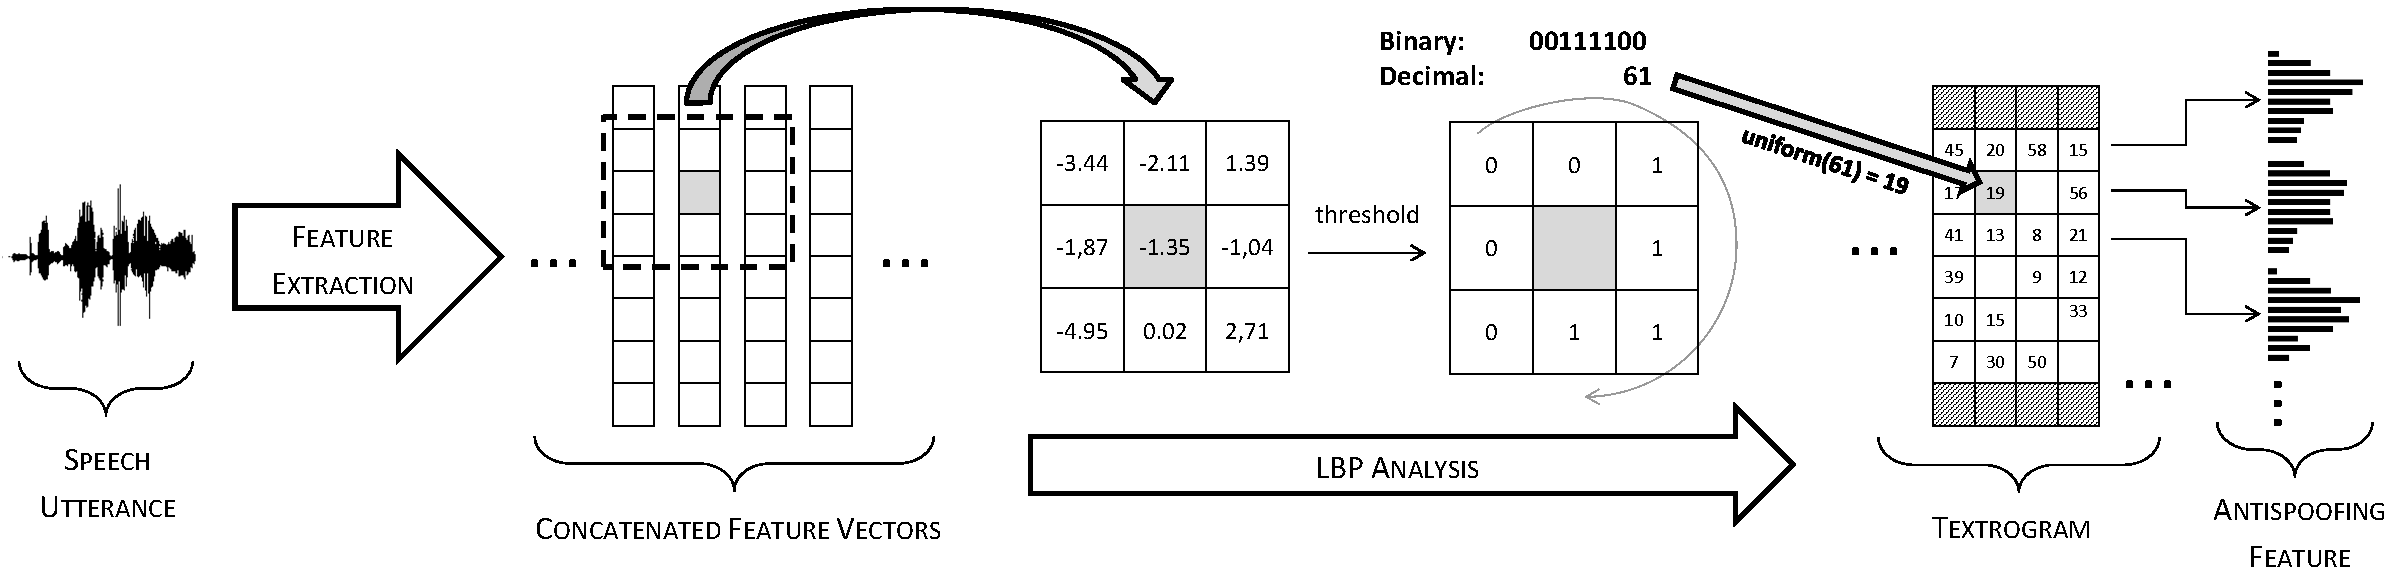
\includegraphics[width=1\linewidth]{Figs/LBPfeature.pdf}

	\caption{Schematic diagram of forming a feature vector in the LBP-based countermeasure.}
	\label{fig:LBPfeature}
\end{figure*}


\subsubsection{FFD setup} The FFD countermeasure was set up according to the algorithm proposed in~\cite{Villalba2011}. Each recording, both from the training and the testing datasets, was additionally described using the following 12 parameters:
\begin{itemize}
\item spectral ratio -- the ratio between
the signal energy from 0 to 2 kHz and from 2 kHz to 4 kHz.  The average value of the spectral ratio for the speech segment was calculated using speech frames only. By using this value we hoped to detect the flattening of the spectrum due to noise and reverberation, caused by far-field recording;
\item low frequency ratio -- ratio between the signal energy from 100 Hz to 300 Hz and from 300 Hz to 500 Hz, calculated using speech frames only. This value is useful for detecting the effect of the loudspeaker on the low part of the spectrum of the replayed signal;
\item total signal modulation index; and
\item nine sub-band modulation indices, for sub-bands: 1kHz-3kHz, 1kHz-2kHz,
2kHz-3kHz, 0.5kHz-1kHz, 1kHz-1.5kHz, 1.5kHz-2kHz, 2kHz-2.5kHz, 2.5kHz-3kHz and 3kHz-3.5kHz.
\end{itemize}

The total modulation index was calculated based on the speech signal's envelope. The envelope was approximated by the absolute value of the signal downsampled to 60 Hz. The average modulation index of the signal was calculated for
the frames whose index was above a threshold of 0.75. According to the authors of the algorithm, the envelope of the far-field recording has higher local minima mainly due to the additive noise, what should result in lower modulation indices. 

Sub-band modulation indices were added to detect far-field recordings disturbed with coloured noises. If a narrow-band noise affected only to a small frequency band it might not have a noticeable effect on the total modulation index.  



\subsubsection{LBP setup} The standard LBP operator is a non-parametric 3x3 kernel which assigns a binary code to each pixel in an image according to the comparison of its intensity value to that of its eight surrounding pixels~\cite{Ojala2002}. This procedure is illustrated in Figure~\ref{fig:LBPfeature}.  A binary value of '1' is assigned when the intensity of neighbouring pixels (here feature components) is higher, whereas a value of '0' is assigned when neighbouring pixels are of lower or equal intensity. Each pixel is thus assigned one of $2^8=256$ binary patterns.

LBPs are determined for each pixel in the mel-scaled cepstrogram thus resulting in a new matrix of reduced dynamic range, here referred to as a 'textrogram'.  The textrogram captures short-time feature motion beyond that in conventional dynamic parametrisation.  The LBP-based countermeasure is based on concatenated histograms formed from the pixel values across each row in the textrogram.  The histograms are individually normalised and their resulting bin values are stacked vertically to obtain a new vector in the same manner as GMM mean-vectors are stacked to form supervectors.  

Compared to the original implementation, we reduced the number of possible patterns according to the standard Uniform LBP approach. Uniform LBPs are the subset of $58$ patterns which contain at most two bitwise transitions from 0 to 1 or 1 to 0 when the bit pattern is traversed in circularly fashion.  As an example, the subset includes patterns $00000001$ and $00111100$ but not $00110001$.  As reported by~\cite{Ojala2002}, most patterns are naturally uniform and empirical evidence suggests that their use in many image recognition applications leads to better performance then the full set of uniform and non-uniform patterns.  We observed similar findings in our previous work~\cite{Alegre2013a} and thus decided to ignore pixels corresponding to any of the 198 non-uniform patterns.

We used the implementation made publicly available by The University of Oulu\footnote{http://www.cse.oulu.fi/CMV/Downloads/LBPMatlab}. Normalised features used in the LBP countermeasure were composed of 51 coefficients: 16 LFCCs and energy plus their corresponding delta and delta-delta coefficients. We took into account only those frames determined to contain speech, i.e. those also used for ASV. Histograms of LBPs are created for all but the first and last frames, thereby obtaining a $58 \times 49 = 2842$ length feature vector.

\subsubsection{Training the replay detectors} Both countermeasure algorithms were trained using a set of 1000 recordings generated using 200 recordings taken from NIST'05 and emulation of various acoustic conditions. In order to make the experiment as close as possible to reality, we decided to use different room impulse responses than the ones used for simulation of replay attack. Therefore we emulated the following environment:
\begin{itemize}
\item a lecture room, with concrete walls, glass windows and a parquet;
\item a staircase, with concrete walls and steps;
\item a meeting room, with concrete walls, glass windows and a carpet.
\end{itemize}

Similarly to emulation of replay attack, the corresponding impulse responses were taken from the AIR database. To train the far-field recording detector, we also needed to emulate the replay device. We chose a stand-alone speaker impulse response, different from the one used for replay attack emulation, to avoid overfitting to testing data. Original NIST'05 recordings were used to model the licit client access trials.

A binary SVM classifier with polynomial kernel of 3rd degree was used for data classification for the FFD countermeasure, while a classifier based on decision table was used for LBP. Those classifiers returned the best results for those two detectors in terms of the area under the ROC curve. Having been trained, both classifiers were applied to detect replay attacks in both spoofing accesses and licit client trials.
